\section{3D-LIP Model with Heading Angles}\label{sec:lip}

\subsection{Local Robot Reference Frame}
The state $\mathbf{x}$ and the input $\mathbf{u}$ of the dynamic model are defined as:

$$ \mathbf{x} := \left( p_x,\; v_x,\; p_y,\; v_y,\; \theta \right)^T \in \mathcal{X} \subset \mathbb{R}^5 , $$
$$ \mathbf{u} := \left( f_x,\; f_y,\; \omega \right)^T \in \mathcal{U} \subset \mathbb{R}^3 , $$

where $(p_x, v_x)$ are the CoM position and translational velocity along the $x$-axis, $f_x$ is the $x$-coordinate of the stance foot position, $\theta$ and $\omega$ are the humanoid's orientation and turning rate, respectively. $\mathcal{X}$ is the set of the allowed states, while $\mathcal{U}$ is the set of the admissible inputs.\\
Both the state and the input are expressed in the local coordinates of the robot, which are time-related. It means that $(p_{x_k}, p_{y_k})$ represents the position of the CoM at simulation time step $k$ in the reference frame ($RF_k$) that originates from $(p_{x_{k-1}}, p_{y_{k-1}})$, and is rotated by an angle $\theta_k$ around the $z$-axis with respect to $RF_{k-1}$. The relation between the vectors in different reference frames is represented in Figure \ref{fig:loc_to_glob_tfm}.\\
The reference frame at time step 0 is considered the "inertial" or "global" frame. A transformation between the inertial and moving frames is necessary to obtain the position of the humanoid in the global map and to deal with obstacles. Transformations are performed as follows:
$$
\mathbf{T_k} = \begin{pmatrix}
\cos\theta_{k,\, \text{glob}} & -\sin\theta_{k,\, \text{glob}} & p_{x,\,k-1,\,\text{glob}} \\
\sin\theta_{k,\, \text{glob}} & \cos\theta_{k,\, \text{glob}} &  p_{y,\,k-1,\,\text{glob}} \\
0 & 0 & 1
\end{pmatrix},
$$

$$
\begin{pmatrix} f_{x,\,k,\,\text{glob} } \\ f_{y,\,k,\,\text{glob}} \\ 1 \end{pmatrix} = \; \mathbf{T_k} \;
\begin{pmatrix}
f_{x,\,k,\,\text{loc} } \\ f_{y,\,k,\,\text{loc}} \\ 1
\end{pmatrix},
$$

$$
\begin{pmatrix} p_{x,\,k,\,\text{glob} } \\ p_{y,\,k,\,\text{glob}} \\ 1 \end{pmatrix} = \; \mathbf{T_k} \;
\begin{pmatrix}
p_{x,\,k,\,\text{loc} } \\ p_{y,\,k,\,\text{loc}} \\ 1
\end{pmatrix},
$$

$$
\begin{pmatrix} v_{x,\,k,\,\text{glob} } \\ v_{y,\,k,\,\text{glob}}\end{pmatrix} = \; \begin{pmatrix} \cos\theta_{k,\, \text{glob}} & -\sin\theta_{k,\, \text{glob}} \\ \sin\theta_{k,\, \text{glob}} & \cos\theta_{k,\, \text{glob}} \end{pmatrix}\;
\begin{pmatrix}
v_{x,\,k,\,\text{loc} } \\ v_{y,\,k,\,\text{loc}}
\end{pmatrix},
$$

$$ 
\theta_{k+1, \text{glob}} = \theta_{k, \text{glob}} + \theta_{k+1, \text{loc}},
\qquad
\omega_{\text{glob}} = \omega_{\text{loc}}.
$$

The positional vectors are roto-translated using a $3\times3$ homogeneous matrix. The velocity vectors are only rotated around the z-axis (indeed, a translation would change their magnitude) using a rotation matrix. The global robot's orientation is obtained by summing the latest local variation to the previous global angle. The angular velocity does not need to be transformed because it is along the $z$-axis, which is fixed.

\begin{figure}[h]
    \centering
    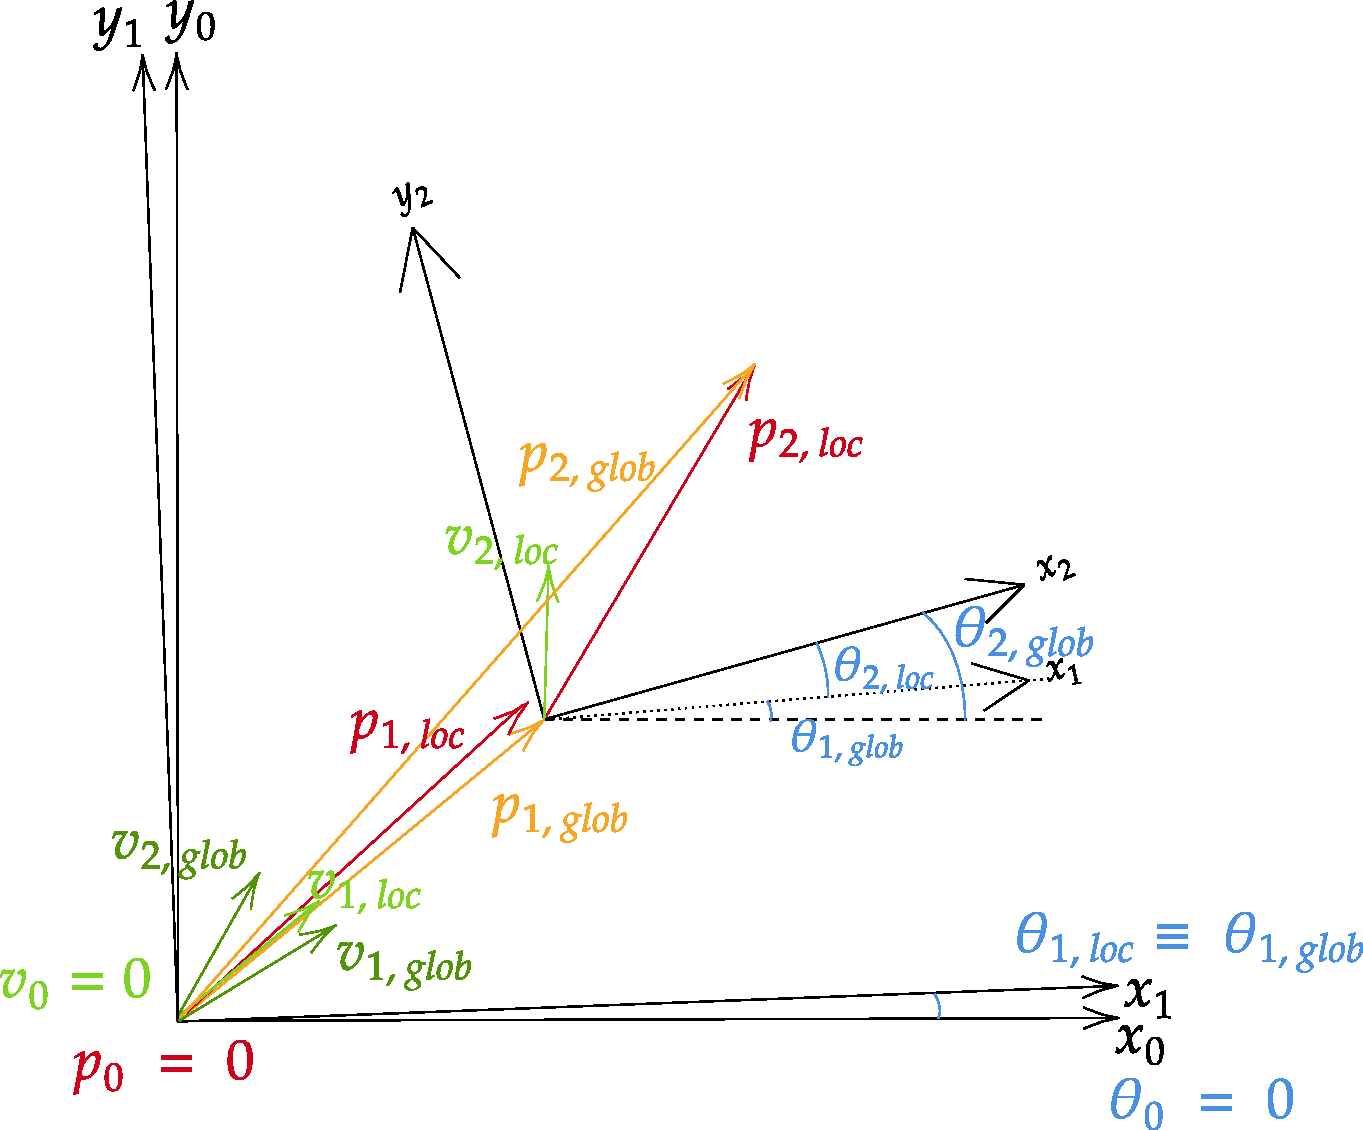
\includegraphics[width=0.75\linewidth]{figures/LIP/loc_to_glob_tfm2.pdf}
    \caption{An example of the evolution of the 3D-LIP model's state, highlighting the relationship between local and global coordinates. The initial state is $\mathbf{0}$ and the RF $(x_0,\, y_0)$ is the inertial frame. The local RF translates and rotates with the simulation time $k$: the position of $RF_2$ $(x_2,\, y_2)$ has its origin in $p_{1, \text{glob}}$, while its orientation is given by $\theta_{2, glob}$. The pose of the successive frames is computed analogously.}
    \label{fig:loc_to_glob_tfm}
\end{figure}

\subsection{Model Definition}
Assuming that the height $H$ of the CoM is constant during the motion, according to \cite{peng_main_paper} we can express the CoM acceleration along the $x$-axis as:
$$
\dot{v}_x = \frac{g}{H}\left(p_x - f_x\right),
$$

with $g$ as the magnitude of the gravitational acceleration. Since by definition $\dot{\theta} \coloneqq \omega$, by Euler integration we obtain that:
$$
\theta_{k+1} = \theta_k + \omega \, T,
$$

where $T$ is the duration of the sampling interval. By further assuming that the duration of a single humanoid's step is fixed and equal to $T$, we can derive the closed-form step-to-step discrete dynamics of the 3D-LIP model:

\begin{equation}\label{eq:lip_dyanmics}
\mathbf{x}_{k+1} = \mathbf{A_L} \, \mathbf{x}_k + \mathbf{B_L} \, \mathbf{u}_k,
\end{equation}
with:
$$
\mathbf{A_L} \coloneqq 
\begin{pmatrix}
\mathbf{A_d} & \mathbf{0} & 0 \\
\mathbf{0} & \mathbf{A_d} & 0 \\
\mathbf{0} & \mathbf{0} & 1 \\
\end{pmatrix}, \qquad
\mathbf{B_L} \coloneqq 
\begin{pmatrix}
\mathbf{B_d} & \mathbf{0} & 0 \\
\mathbf{0} & \mathbf{B_d} & 0 \\
0 & 0 & T
\end{pmatrix},
$$
$$
\mathbf{A_d} \coloneqq 
\begin{pmatrix}
\cosh{\beta \, T} & \frac{\sinh{\beta \, T}}{\beta}  \\
\beta \, \sinh{\beta \, T} & \cosh{\beta \, T}
\end{pmatrix}, \qquad
\mathbf{B_d} \coloneqq 
\begin{pmatrix}
1 - \cosh{\beta \, T} \\
-\beta \, \sinh{\beta \, T}
\end{pmatrix}, \qquad
\beta \coloneqq \sqrt{\frac{g}{H}}
$$
\\
In the following chapter, these dynamics will be used as the internal process representation of an MPC. Along with the constraints, they will grant that the found solution is meaningful to the humanoid motion.


\section{3D-LIP Model with Heading Angles}
Due to the high dimensionality and non-linearity of the full dynamic model of a humanoid, we have used a simplified model base on the standard Linear Inverted Pendulum formulation.
This reduced model assumes that during the motion, the Center of Mass (CoM) will have a constant height during the motion.
According to (citation), we can express the acceleration of the CoM position as follows:
\begin{align}
    \begin{cases}
        \dot{v}_{x} = \frac{g}{H}(p_{x} - f_{x})
        \\[1ex]
        \dot{v}_{y} = \frac{g}{H}(p_{y} - f_{y})
    \end{cases}
\end{align}

with $(p_{x}, p_{y})$ we denote the position of the CoM and with $(v_{x}, v_{y})$ its velocity with respect to the $x$-axis and $y$-axis. The stance foot position, which is the position in which both feets are in contact with the ground, is denoted with $(f_{x}, f_{y})$.

By defining the state of our system as $x = [p_{x}, v_{x}, p_{y}, v_{y}, \theta]^T \in \mathbb{R}^5$ and the control input as $u = [f_{x}, f_{y}, \omega]^T \in \mathbb{R}^3$, where $\theta$ is the heading angle and $\omega$ is its turning rate, the dynamics of the model can be written as follows:
\begin{equation}
    \dot{x}(t) = A x(t) + B u(t)
\end{equation}
This equation can be expanded as:
\begin{align}
    \dot{x} = 
    \begin{bmatrix}
        \dot{p}_{x}\\
        \dot{v}_{x}\\
        \dot{p}_{y}\\
        \dot{v}_{y}\\
        \dot{\theta}
    \end{bmatrix}
    &=
    \begin{bmatrix}
        0 & 1 & 0 & 0 & 0 \\[1ex]
        \frac{g}{H} & 0 & 0 & 0 & 0 \\[1ex]
        0 & 0 & 0 & 1 & 0 \\[1ex]
        0 & 0 & \frac{g}{H} & 0 & 0 \\[1ex]
        0 & 0 & 0 & 0 & 0
    \end{bmatrix}
    \begin{bmatrix}
        p_{x}\\
        v_{x}\\
        p_{y}\\
        v_{y}\\
        \theta
    \end{bmatrix}
    +
    \begin{bmatrix}
        0 & 0 & 0 \\[1ex]
        -\frac{g}{H} & 0 & 0 \\[1ex]
        0 & 0 & 0 \\[1ex]
        0 & -\frac{g}{H} & 0 \\[1ex]
        0 & 0 & 1 \\[1ex]
    \end{bmatrix}
    \begin{bmatrix}
        f_{x} \\
        f_{y} \\
        \omega
    \end{bmatrix}
    =
    \\
    &= 
    \begin{bmatrix}
        A_c & 0 & 0 \\
        0 & A_c & 0 \\
        0 & 0 & 0
    \end{bmatrix}
    x(t) +
    \begin{bmatrix}
        B_c & 0 & 0 \\
        0 & B_c & 0 \\
        0 & 0 & 0
    \end{bmatrix}
    u(t)
\end{align}
where $A_{c} \in \mathbb{R}^{2 \times 2}$, $B_{c} \in \mathbb{R}^{2 \times 1}$ and $\beta = \sqrt{\frac{g}{H}}$.
\\
From this continuous model, we can obtain the following discretized system: 
\begin{equation}
    x_{k+1} = A_{L}x_{k} + B_{L}u_{k}
\end{equation}
where the two matrices are defined as:

\begin{align}
    A_{L} = 
    \begin{bmatrix}
        A_{d} & 0 & 0 \\
        0 & A_{d} & 0 \\
        0 & 0 & 1
    \end{bmatrix}
    \qquad
    B_{d} = 
    \begin{bmatrix}
        B_{d} & 0 & 0 \\
        0 & B_{d} & 0 \\
        0 & 0 & T
    \end{bmatrix}
\end{align}

with:
\begin{equation}
    A_{d} = 
    \begin{bmatrix}
        cosh(\beta T) & \frac{sinh(\beta T)}{\beta} \\
        \beta sinh(\beta T) & cosh(\beta T)
    \end{bmatrix}
    \qquad
    B_{d} = 
    \begin{bmatrix}
        1 - cosh(\beta T) \\
        - \beta sinh(\beta T)
    \end{bmatrix}
\end{equation}

\todo[inline]{improve the discretization part}